\let\negmedspace\undefined
\let\negthickspace\undefined
\documentclass[journal]{IEEEtran}
\usepackage[a5paper, margin=10mm, onecolumn]{geometry}
%\usepackage{lmodern} % Ensure lmodern is loaded for pdflatex
\usepackage{tfrupee} % Include tfrupee package

\setlength{\headheight}{1cm} % Set the height of the header box
\setlength{\headsep}{0mm}     % Set the distance between the header box and the top of the text

\usepackage{gvv-book}
\usepackage{gvv}
\usepackage{cite}
\usepackage{amsmath,amssymb,amsfonts,amsthm}
\usepackage{algorithmic}
\usepackage{graphicx}
\usepackage{textcomp}
\usepackage{xcolor}
\usepackage{txfonts}
\usepackage{listings}
\usepackage{enumitem}
\usepackage{mathtools}
\usepackage{gensymb}
\usepackage{comment}
\usepackage[breaklinks=true]{hyperref}
\usepackage{tkz-euclide} 
\usepackage{listings}
% \usepackage{gvv}                                        
\def\inputGnumericTable{}                                 
\usepackage[latin1]{inputenc}                                
\usepackage{color}                                            
\usepackage{array}                                            
\usepackage{longtable}                                       
\usepackage{calc}                                             
\usepackage{multirow}                                         
\usepackage{hhline}                                           
\usepackage{ifthen}                                           
\usepackage{lscape}
\begin{document}

\bibliographystyle{IEEEtran}
\vspace{3cm}

\title{CHAPTER - 9\\Intersection of Conics}
\author{EE24BTECH11061 - Rohith Sai}
% \maketitle
% \newpage
% \bigskip
{\let\newpage\relax\maketitle}

\renewcommand{\thefigure}{\theenumi}
\renewcommand{\thetable}{\theenumi}
\setlength{\intextsep}{10pt} % Space between text and floats

\numberwithin{figure}{enumi}
\renewcommand{\thetable}{\theenumi}

\section{9.3 CBSE}
\begin{enumerate}
\item [9.3.22] If the area between the curves $x=y^2$ and $x=4$ is divided into two equal parts by the line $x=a$, then find the value of $a$, using integration.\\
\textbf{Solution:}\\
The given conic parameters are
\begin{align}
    \vec{V} = \myvec{0 & 0\\0 & 1}, \vec{u} = \frac{-1}{2}\vec{e_1}, f = 0
\end{align}
The parameters of the line $x=a$ are
\begin{align}
    \vec{q_2} = \myvec{a\\0}, \vec{m_2} = e_2
\end{align}
We get
\begin{align}
    \mu_i = -\sqrt{a},\sqrt{a}
\end{align}
The points of intersection of the line $x=a$ with the parabola $x=y^2$ is 
\begin{align}
    \vec{a_0} = \myvec{a\\-\sqrt{a}}, \vec{a_1} = \myvec{a\\\sqrt{a}}
\end{align}
Similarly for the line $x-4=0$
\begin{align}
    \vec{q_1} = \myvec{4\\0}, \vec{m_1} = e_2
\end{align}
We get
\begin{align}
    \mu_i = -2,2
\end{align}
The points of intersection of the lines $x=4$ with the parabola $x=y^2$ is
\begin{align}
    \vec{a_2} = \myvec{4\\-2}, \vec{a_3} = \myvec{4\\2}
\end{align}
Area between the parabola and the line $x=4$ is divided equally by the line $x=a$. Thus from Fig. 9.3.22.1,
\begin{align}
    A_1 = \int_0^a \sqrt{x}, dx\\
    A_2 = \int_a^4 \sqrt{x}, dx\\
    \text{and } A_1 = A_2\\
    \implies a = 4^{\frac{2}{3}}
\end{align}
Therefore, we get the following graph
\begin{figure}[h!]
    \centering
    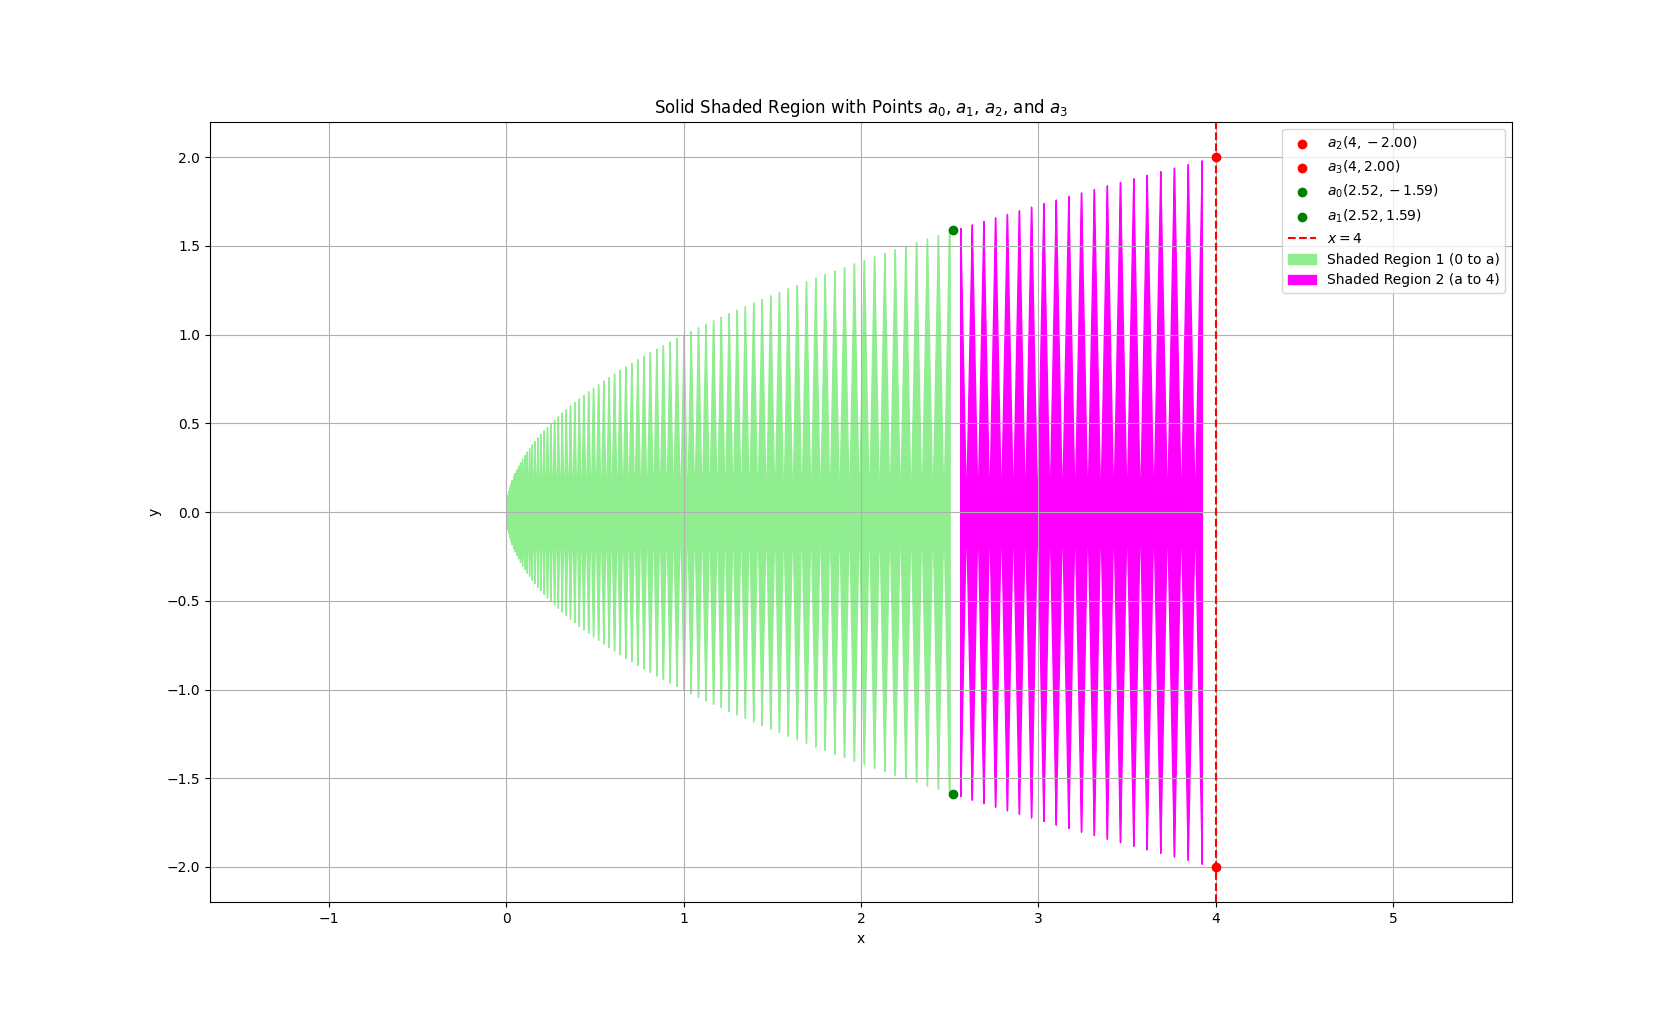
\includegraphics[width=9.5cm]{figs/figure.png}
    \caption*{Fig. 9.3.22.1}
    \label{}
\end{figure}
\end{enumerate}
\end{document}